\documentclass[12pt, twoside]{book}

\usepackage[a4paper,top=2.5cm,bottom=2.5cm,left=3.5cm,right=2cm]{geometry}
\usepackage[utf8]{inputenc}
\usepackage[T1]{fontenc}

\usepackage[slovak]{babel}
\usepackage[babel]{csquotes}

  \linespread{1.25}

\usepackage{listings}
\lstset{frame=lines}

\usepackage{graphicx}
\usepackage{pdfpages}
\usepackage{url}
\usepackage[hidelinks,breaklinks]{hyperref}
\usepackage{dirtytalk}

\def\mfrok{2024}
\def\mfnazov{Systém na podporu vypracovania bezpečnostných projektov pre malé ISVS}
\def\mftyp{Bakalárska práca}
\def\mfautor{Anton Kica}
\def\mfskolitel{doc. RNDr. Daniel Olejár, PhD.}
\def\mfmiesto{Bratislava, \mfrok}
\def\mfodbor{Informatika}
\def\program{Informatika}
\def\mfpracovisko{Katedra informatiky}

\begin{document}     
\frontmatter
\pagestyle{empty}

% -------------------
% --- Obalka ------
% -------------------

\begin{center}
\sc\large
Univerzita Komenského v Bratislave\\
Fakulta matematiky, fyziky a informatiky

\vfill

{\LARGE\mfnazov}\\
\mftyp
\end{center}

\vfill

{\sc\large 
\noindent \mfrok\\
\mfautor
}

\cleardoublepage
% --- koniec obalky ----

% -------------------
% --- Titulný list
% -------------------


\noindent

\begin{center}
\sc  
\large
Univerzita Komenského v Bratislave\\
Fakulta matematiky, fyziky a informatiky

\vfill

{\LARGE\mfnazov}\\
\mftyp
\end{center}

\vfill

\noindent
\begin{tabular}{ll}
Študijný program: & \program \\
Študijný odbor: & \mfodbor \\
Školiace pracovisko: & \mfpracovisko \\
Školiteľ: & \mfskolitel \\
\end{tabular}

\vfill


\noindent \mfmiesto\\
\mfautor

\cleardoublepage
% --- Koniec titulnej strany


% -------------------
% --- Zadanie z AIS
% -------------------
% v tlačenej verzii s podpismi zainteresovaných osôb.
% v elektronickej verzii sa zverejňuje zadanie bez podpisov
% v pracach v angličtine anglické aj slovenské zadanie

\newpage 
\setcounter{page}{3}
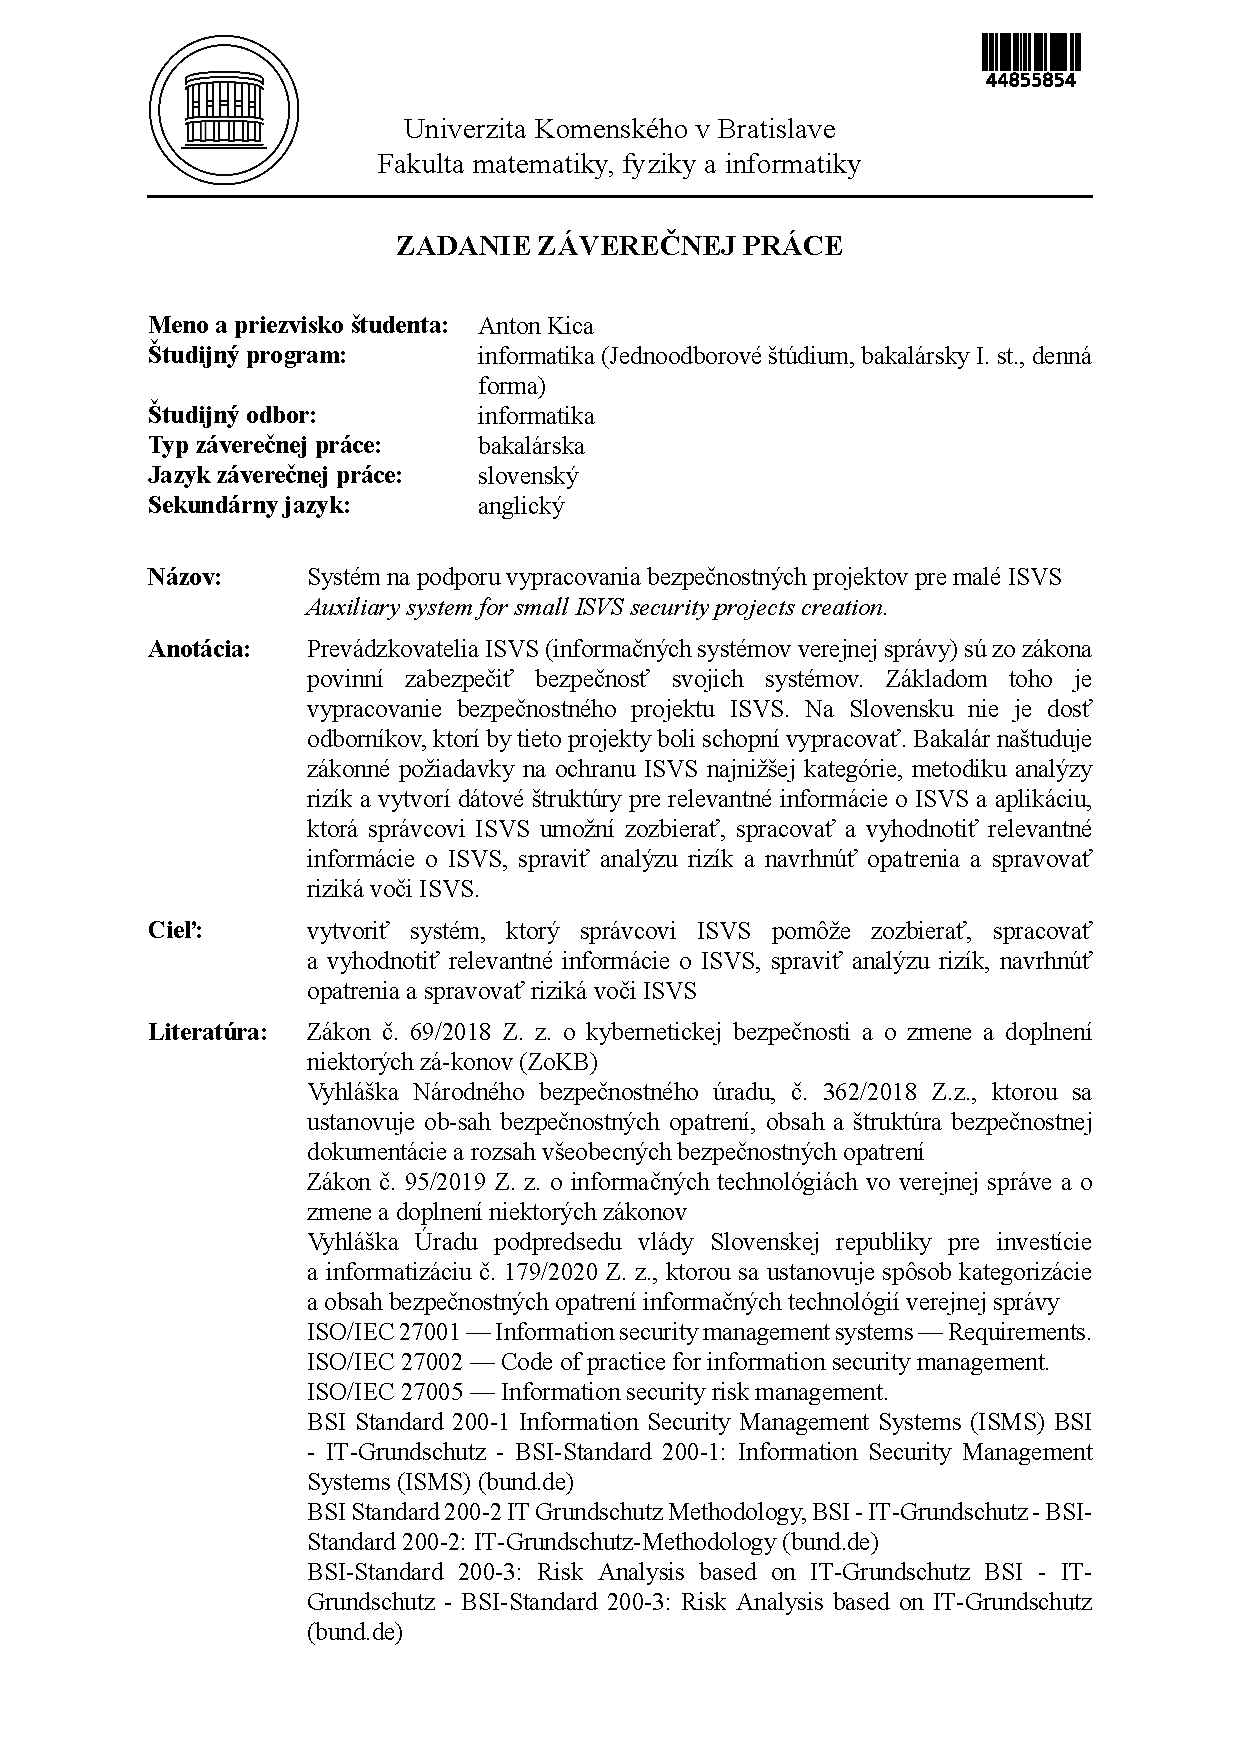
\includepdf{images/zadanie.pdf}

% --- Koniec zadania


% -------------------
%   Poďakovanie - nepovinné
% -------------------
\newpage 
\pagestyle{plain}
~

\vfill
{\bf Poďakovanie:} Ešte nie je komu.

% --- Koniec poďakovania

% -------------------
%   Abstrakt - Slovensky
% -------------------
\newpage 
\section*{Abstrakt}

Aké výsledky?

\paragraph*{Kľúčové slová:} 
kybernetická a informačná bezpečnosť,
ISVS,
bezpečnostnýs projekt,
analýza rizík,
správa rizík
% --- Koniec Abstrakt - Slovensky


% -------------------
% --- Abstrakt - Anglicky 
% -------------------
\newpage 
\section*{Abstract}

What results?

\paragraph*{Keywords:} 
cybernetics and information security,
ISVS,
security project,
risk analysis,
risk managment

% --- Koniec Abstrakt - Anglicky

% -------------------
% --- Obsah
% -------------------


\cleardoublepage
\tableofcontents

% ---  Koniec Obsahu

% -------------------
% --- Zoznamy tabuliek, obrázkov - nepovinne
% -------------------

\newpage 

\listoffigures
\listoftables

% ---  Koniec Zoznamov

\mainmatter
\pagestyle{headings}


\input ./00-uvod.tex

\input ./10-problematika.tex

\input ./20-zaver.tex

    % \input ./praca/latex.tex
% \input ./praca/kapitola.tex

% -------------------
% --- Bibliografia
% -------------------


\newpage	

\backmatter

\thispagestyle{empty}
\clearpage

\bibliographystyle{plain}
\bibliography{literatura} 

%---koniec Referencii

% -------------------
%--- Prilohy---
% -------------------

%Nepovinná časť prílohy obsahuje materiály, ktoré neboli zaradené priamo  do textu.
%Každá príloha sa začína na novej strane.
%Zoznam príloh je súčasťou obsahu.
%

\end{document}
